\begin{figure}[h!]
\small
\begin{center}
\setlength{\tabcolsep}{1pt}
\begin{tabular}{ccccc}
 &&
&\hspace{-30mm} 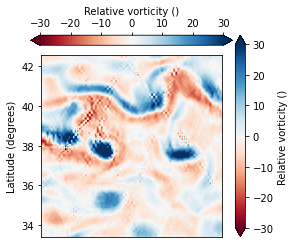
\includegraphics[trim={8mm 7cm 22mm 0},clip,width=5.0cm,height=1cm]{figures/plots/horizontal_cbar_vort.png} &\\
\hspace{0mm} &&
\hspace{-30mm} Training  
\hspace{3mm}  & 
 & 
\hspace{-30mm} Reconstruction \\

%\vspace{-2mm}
%%%%% ORCA025 %%%%%%%%

\hspace{-10mm}  1)&
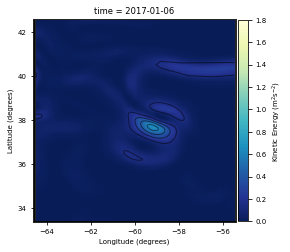
\includegraphics[trim={0 13mm 22mm 5mm},clip, width=3.60cm,height=3.2cm]{figures/plots/orca025_train_ke.png} &
 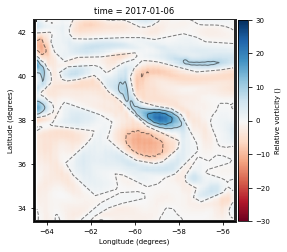
\includegraphics[trim={13mm 13mm 22mm 5mm},clip, width=3.2cm,height=3.2cm]{figures/plots/orca025_train_vort_r.png} &
 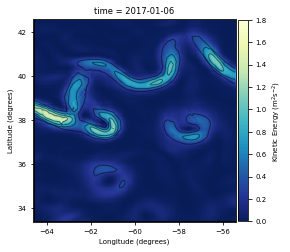
\includegraphics[trim={13mm 13mm 22mm 5mm},clip, width=3.2cm,height=3.2cm]{figures/plots/orca025_rec_ke.png} &
 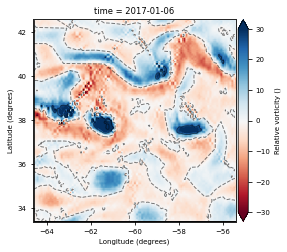
\includegraphics[trim={13mm 13mm 22mm 5mm},clip,width=3.2cm,height=3.2cm]{figures/plots/orca025_rec_vort_r.png} \\
%\vspace{3mm}
%%%%% GLORYS12-f %%%%%%%%
\hspace{-10mm} 2) &
 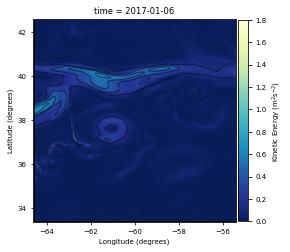
\includegraphics[trim={0 13mm 22mm 5mm},clip, width=3.60cm,height=3.2cm]{figures/plots/glorys12-f_train_ke.png} &
 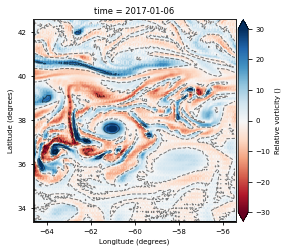
\includegraphics[trim={13mm 13mm 22mm 5mm},clip, width=3.2cm,height=3.2cm]{figures/plots/glorys12-f_train_vort_r.png} &
 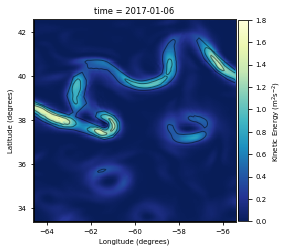
\includegraphics[trim={13mm 13mm 22mm 5mm},clip, width=3.2cm,height=3.2cm]{figures/plots/glorys12-f_rec_ke.png} &
 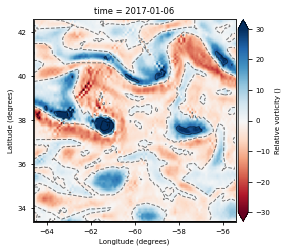
\includegraphics[trim={13mm 13mm 22mm 5mm},clip,width=3.2cm,height=3.2cm]{figures/plots/glorys12-f_rec_vort_r.png} \\
%\vspace{3mm}
%%%%% GLORYS12-f %%%%%%%%
\hspace{-10mm} 3) &
 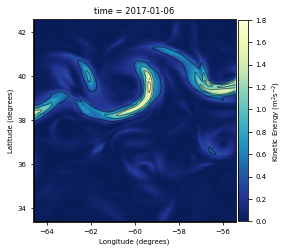
\includegraphics[trim={0 13mm 22mm 5mm},clip, width=3.60cm,height=3.2cm]{figures/plots/glorys12-r_train_ke.png} &
 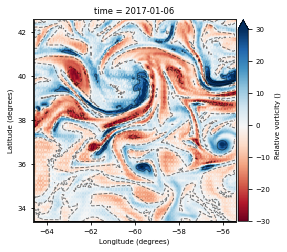
\includegraphics[trim={13mm 13mm 22mm 5mm},clip, width=3.2cm,height=3.2cm]{figures/plots/glorys12-r_train_vort_r.png} &
 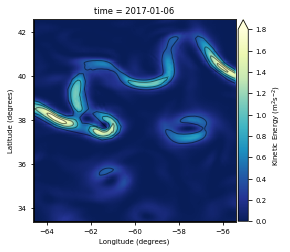
\includegraphics[trim={13mm 13mm 22mm 5mm},clip, width=3.2cm,height=3.2cm]{figures/plots/glorys12-r_rec_ke.png} &
 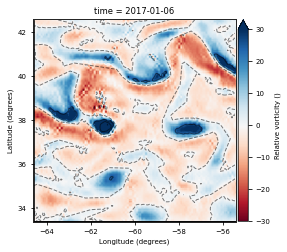
\includegraphics[trim={13mm 13mm 22mm 5mm},clip,width=3.2cm,height=3.2cm]{figures/plots/glorys12-r_rec_vort_r.png} \\
%%%%% NATL60 %%%%%%%%
\hspace{-10mm} 4) &
 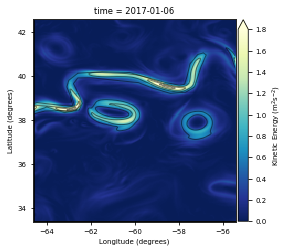
\includegraphics[trim={0 13mm 22mm 5mm},clip, width=3.60cm,height=3.2cm]{figures/plots/natl60_train_ke.png} &
 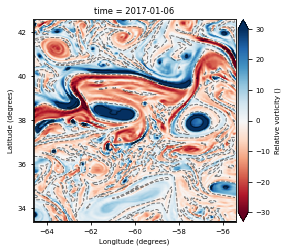
\includegraphics[trim={13mm 13mm 22mm 5mm},clip, width=3.2cm,height=3.2cm]{figures/plots/natl60_train_vort_r.png} &
 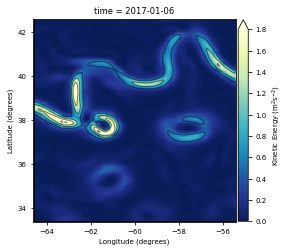
\includegraphics[trim={13mm 13mm 22mm 5mm},clip, width=3.2cm,height=3.2cm]{figures/plots/natl60_rec_ke.png} &
 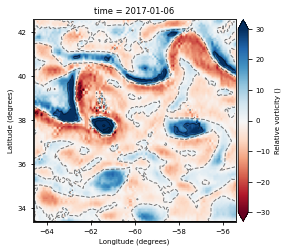
\includegraphics[trim={13mm 13mm 22mm 5mm},clip,width=3.2cm,height=3.2cm]{figures/plots/natl60_rec_vort_r.png} \\
%\vspace{3mm}
%%%%% eNATL60-t %%%%%%%%
\hspace{-10mm} 5) &
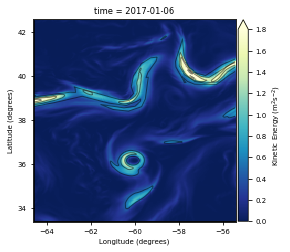
\includegraphics[trim={0 13mm 22mm 5mm},clip, width=3.60cm,height=3.2cm]{figures/plots/enatl60-t_train_ke.png} &
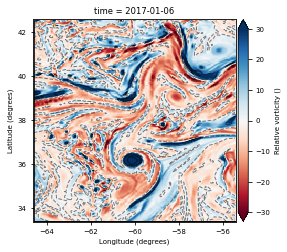
\includegraphics[trim={13mm 13mm 22mm 5mm},clip, width=3.2cm,height=3.2cm]{figures/plots/enatl60-t_train_vort_r.png} &
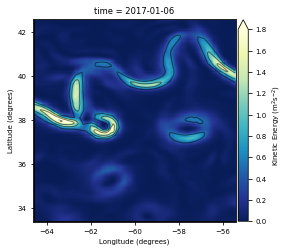
\includegraphics[trim={13mm 13mm 22mm 5mm},clip, width=3.2cm,height=3.2cm]{figures/plots/enatl60-t_rec_ke.png} &
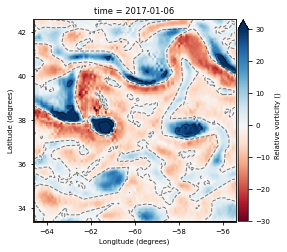
\includegraphics[trim={13mm 13mm 22mm 5mm},clip,width=3.2cm,height=3.2cm]{figures/plots/enatl60-t_rec_vort_r.png} \\
%\vspace{3mm}
%%%%% eNATL60-0 %%%%%%%%
\hspace{-10mm} 6) &
 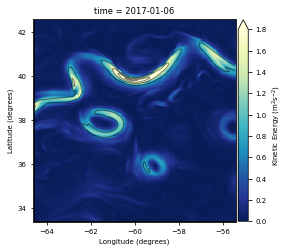
\includegraphics[trim={0 0 19mm 5mm},clip, width=3.60cm,height=3.4cm]{figures/plots/enatl60-0_train_ke.png} &
 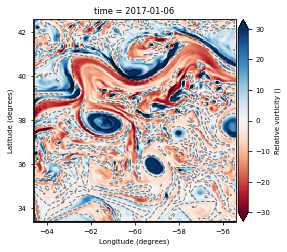
\includegraphics[trim={13mm 0 22mm 5mm},clip, width=3.2cm,height=3.4cm]{figures/plots/enatl60-0_train_vort_r.png} &
 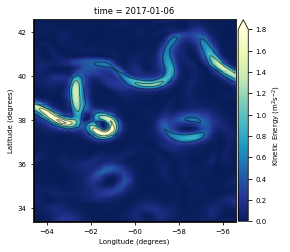
\includegraphics[trim={13mm 0 22mm 5mm},clip, width=3.2cm,height=3.4cm]{figures/plots/enatl60-0_rec_ke.png} &
 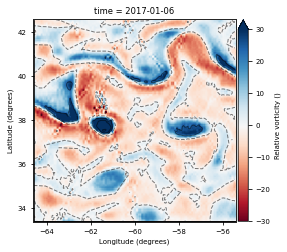
\includegraphics[trim={13mm 0 22mm 5mm},clip,width=3.2cm,height=3.4cm]{figures/plots/enatl60-0_rec_vort_r.png} \\
 \hspace{-15mm} &(a) & (b) & (c) & (d) \\
 &&
&\hspace{-30mm} 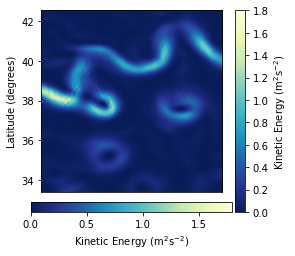
\includegraphics[trim={8mm 0 22mm 7cm},clip,width=4.5cm,height=1cm]{figures/plots/horizontal_cbar_ke_bottom.png} &\\
% \vspace{-2mm}

\end{tabular}
\vspace{-3mm}
% \caption{Row I - Isotrophic PSD. Row 2 - Isotrophic PSD Score}
\caption{
Kinetic energy ((a) and (b) and relative vorticity ((c) and (d)) of the training dataset ((a) and (c)) and the associated 4dVarNet reconstructions ((b) and (d)) at the 6th of January.
Each row shows the experiment using: 1) ORCA025, 2) GLORYS12-f, 3) GLORYS12-r, 4) NATL60, 5) eNATL60-t, eNATL60-0}
\vspace{-5mm}
\label{fig:maps}
\end{center}
\end{figure}